\subsection{Generazione di immagini}

Ultimato l'addestramento della U-Net, si possono sfruttare le transizioni~\eqref{eq:chain_transition132} della catena markoviana 
della diffusione inversa per rimuovere iterativamente il rumore.

In particolare, poiché la versione approssimata $\bm{\mu}_{\bm{\theta}}(\mathbf{x}_t,t)$, dalla rete neurale,
della media~\eqref{eq:true_mean} $\tilde{\bm{\mu}}_t(\mathbf{x}_t)$ è:
\begin{equation}
  \bm{\mu}_{\bm{\theta}}(\mathbf{x}_t,t)=\frac{1}{\sqrt{\alpha_t}}\biggl(\mathbf{x}_t-\frac{1-\alpha_t}{\sqrt{1-\overline{\alpha}_t}}\bm{\epsilon}_{\bm{\theta}}(\mathbf{x}_t,t)\biggr)\label{eq:learned_mean1}
\end{equation}
combinando la~\eqref{eq:learned_mean1} con la~\eqref{eq:chain_transition132}, e sfruttando l'artificio di riparametrizzazione~\eqref{eq:rep_trick}, risulta che 
\begin{equation}
  \mathbf{x}_{t-1}=\frac{1}{\sqrt{\alpha_t}}\biggl(\mathbf{x}_t-\frac{1-\alpha_t}{\sqrt{1-\overline{\alpha}_t}}\bm{\epsilon}_{\bm{\theta}}(\mathbf{x}_t,t)\biggr)+
  \sqrt{\beta_t}\bm{\epsilon} \label{eq:sampling}
\end{equation}
dove $\bm{\epsilon}$ è una gaussiana standard. 
Applicando ricorsivamente la formula~\eqref{eq:sampling} è possibile risalire, partendo da $\mathbf{x}_T$ 
(che è indistinguibile dal rumore puro), all'immagine di partenza $\mathbf{x}_0$ (Figura~\ref{fig:sampling}).

\medskip
\begin{oss}
A scopo puramente chiarificatore, si consideri, ad esempio, il passo $t=50$. 
Nella diffusione inversa il rumore $\bm{\epsilon}_{\bm{\theta}}(\mathbf{x}_{50},50)$, stimato dalla Unet, 
è il rumore che sottratto a $\mathbf{x}_{50}$ restituisce $\mathbf{x}_0$ non $\mathbf{x}_{49}$. 
Tuttavia, da un'attenta analisi della formula~\eqref{eq:sampling}, 
ciò che si sottrae a $\mathbf{x}_{50}$, per ottenere $\mathbf{x}_{49}$, è una versione scalata, 
del fattore $(1-\alpha_t)/\sqrt{1-\overline{\alpha}_t}$, di tale rumore.
\end{oss}

\smallskip
\begin{oss}
Avendo Ho et al.~\cite{ho2020} scelto uno schema di diffusione lineare, cosicché i $\beta_t$ si incrementano linearmente, 
e considerando le definizioni~\eqref{eq:alphas} di $\alpha_t$ e $\overline{\alpha}_t$, dalla formula~\eqref{eq:sampling} si evince che 
il primo passo della diffusione inversa sottrae da $\mathbf{x}_T$ soltanto una piccola parte del rumore $\bm{\epsilon}_{\bm{\theta}}(\mathbf{x}_t,t)$ stimato dalla U-Net.
Viceversa, i passi di diffusione inversa successivi sottraggono da $\mathbf{x}_t$ aliquote del rumore stimato dalla rete neurale via via sempre più grandi.
\end{oss}

\begin{figure}
\centering
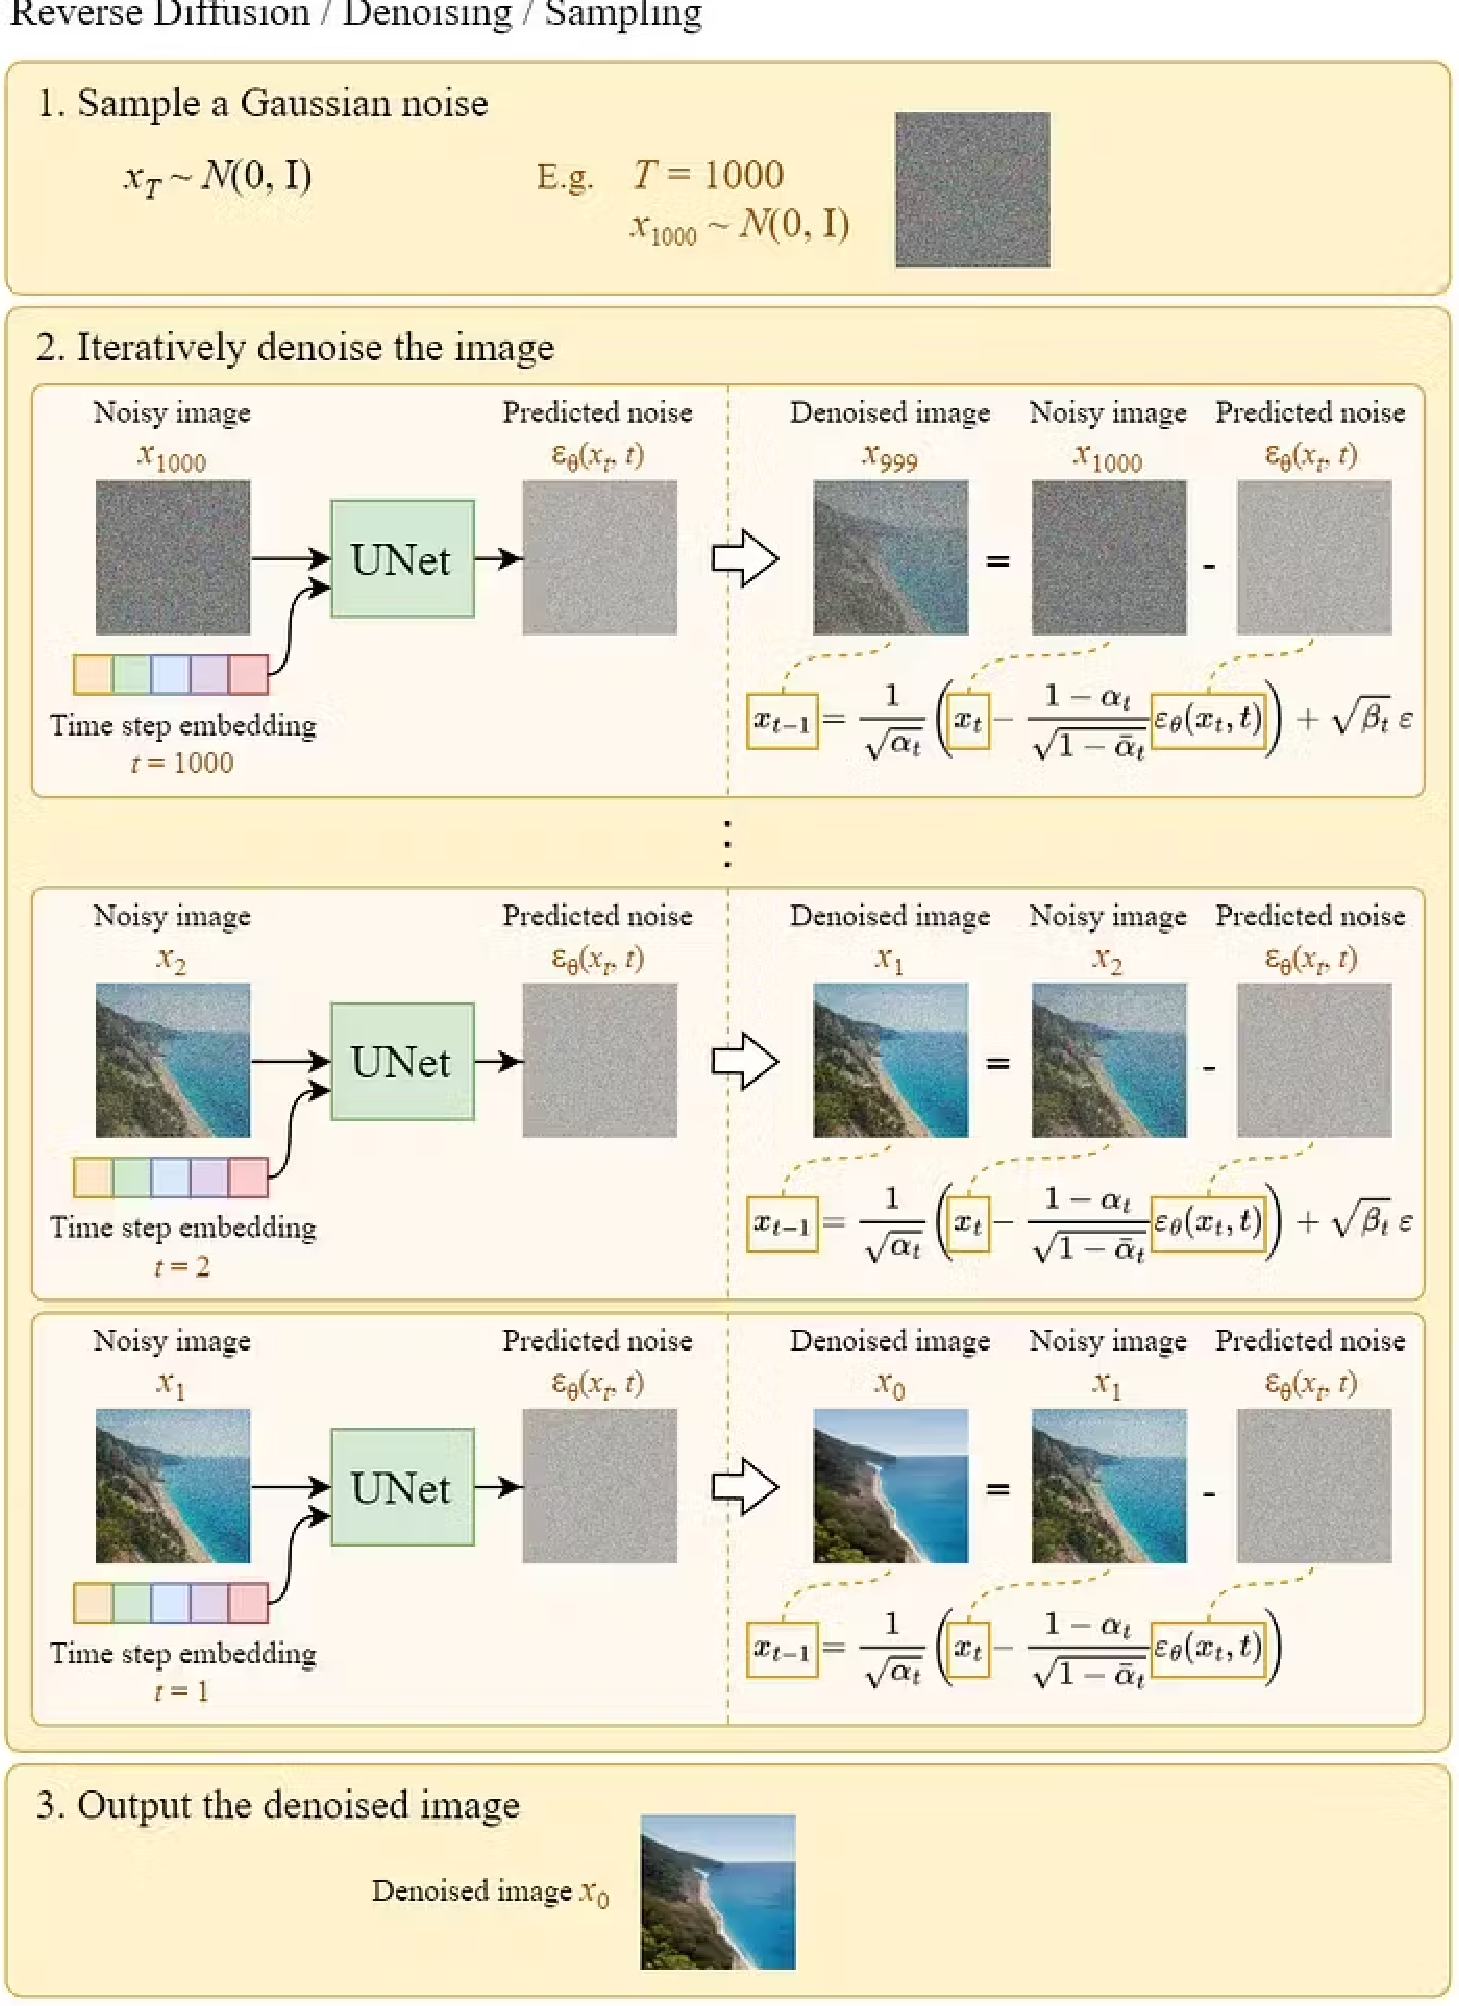
\includegraphics[keepaspectratio, scale=0.55]{sampling1.pdf}
\caption{Generazione di immagini con il processo di diffusione inversa. Fonte~\cite{royBeginnerGuideDiffusion}.}
\label{fig:sampling}
\end{figure}


\begin{algorithm}
    \caption{Generazione di immagini. Fonte~\cite{ho2020}}\label{alg:sampling}
   \begin{algorithmic}[1]
    \State $\mathbf{x}_T\sim\mathcal{N}(\bm{0},\bm{I})$
    \State \textbf{for} $t=T,\dots,1$ \textbf{do}
      \State \hspace{2em}$\mathbf{\bm{\epsilon}}\sim\mathcal{N}(\bm{0},\bm{I})$ if $t>1$, else $\mathbf{\bm{\epsilon}}=\bm{0}$
      \State \hspace{2em}$\mathbf{x}_{t-1}=\frac{1}{\sqrt{\alpha_t}}\biggl(\mathbf{x}_t-\frac{1-\alpha_t}{\sqrt{1-\overline{\alpha}_t}}\bm{\epsilon}_{\bm{\theta}}(\mathbf{x}_t,t)\biggr)+\sqrt{\beta_t}\mathbf{\bm{\epsilon}}$
    \State \textbf{end for}
    \State \textbf{return} $\mathbf{x}_0$
   \end{algorithmic}
\end{algorithm}